\documentclass[a4paper,12pt]{article}
\usepackage{cmap}
\usepackage[utf8]{inputenc}
\usepackage[warn]{mathtext}
\usepackage{epsf,amsmath,amsfonts,amssymb,amsbsy}
\usepackage[mathscr]{eucal}
\usepackage[english, russian]{babel}
\usepackage[left=2cm,right=2cm,top=2cm,bottom=2cm]{geometry}
\usepackage{graphicx}
\usepackage{indentfirst}
\graphicspath{{picture/}}
\DeclareGraphicsExtensions{.pdf,.png,.jpg}
\usepackage{pgfplots}
\usepackage{rotating}
\usepackage{pgfplotstable}
\usepackage{booktabs}
\usepackage{xcolor}
\usepackage{hyperref}
\usepackage{multirow}
\begin{document}

% начало документа
% НАЧАЛО ТИТУЛЬНОГО ЛИСТА
\begin{center}
	\hfill \break
	\hfill \break
	{\small ФЕДЕРАЛЬНОЕ ГОСУДАРСТВЕННОЕ АВТОНОМНОЕ ОБРАЗОВАТЕЛЬНОЕ\\ УЧРЕЖДЕНИЕ ВЫСШЕГО ОБРАЗОВАНИЯ\\ МОСКОВСКИЙ ФИЗИКО-ТЕХНИЧЕСКИЙ ИНСТИТУТ\\ (НАЦИОНАЛЬНЫЙ ИССЛЕДОВАТЕЛЬСКИЙ УНИВЕРСИТЕТ)\\ ФИЗТЕХ-ШКОЛА РАДИОТЕХНИКИ И КОМПЬЮТЕРНЫХ ТЕХНОЛОГИЙ}\\

	\hfill \break
	\normalsize{Лабораторная работа по программированию. }\\
	\vspace{7em}
	\normalsize{\textbf{По теме}}\\
	\vspace{7em}
	\large{<<Исследование эффективности работы хэш-функций>>}\\
\end{center}

\vspace{16em}
\begin{flushright}
	\normalsize{Студента 1 курса группы Б01-003}\\
	\normalsize{\textbf{Крейнина Матвея Вадимовича}}\\
\end{flushright}

\vspace{\fill}
\begin{center}
	\normalsize{\textbf{Долгопрудный, 2021}}
\end{center}


\thispagestyle{empty} % выключаем отображение номера для этой страницы
\newpage
% КОНЕЦ ТИТУЛЬНОГО ЛИСТА

	
	\begin{center}
		{\Large Исследование эффективности работы хэш-функций}
	\end{center}
	\section*{Анотация}
\noindent \textbf{Цель работы:} \\
\indent Сравнение эффективности работы различных хэш-функций, а именно:

\begin{enumerate}
\item best-hash
\item first-sym-hash
\item len-hash
\item sum-hash
\item worst-hash
\item ly-hash
\item rot-13
\end{enumerate}


\section*{В работе используются}
Кривые руки Матвея Крейнина, классы list и line, написанные им же в 1-м семестре, хорошее настроение и любовь к программированию.

\section*{Теоретическое введение}

Это секретная информация, которую нельзя разглашать.
Возможно, вы сможете найти ответ в книге человека, которого нельзя называть.

\section*{Результаты измерений и обработка данных}

\begin{figure}[h]
	\center{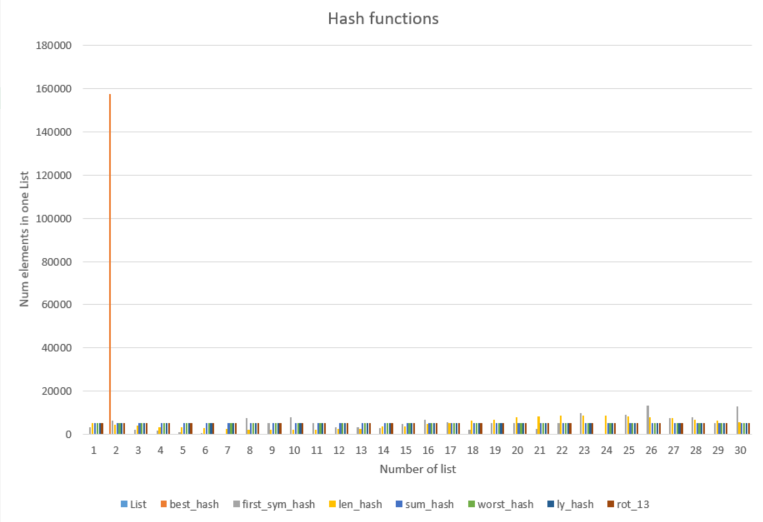
\includegraphics[scale=1]{1}}
	\caption{Измерение, сделанной с лучшей функцией best-hash}
\end{figure}

\begin{figure}[h]
	\center{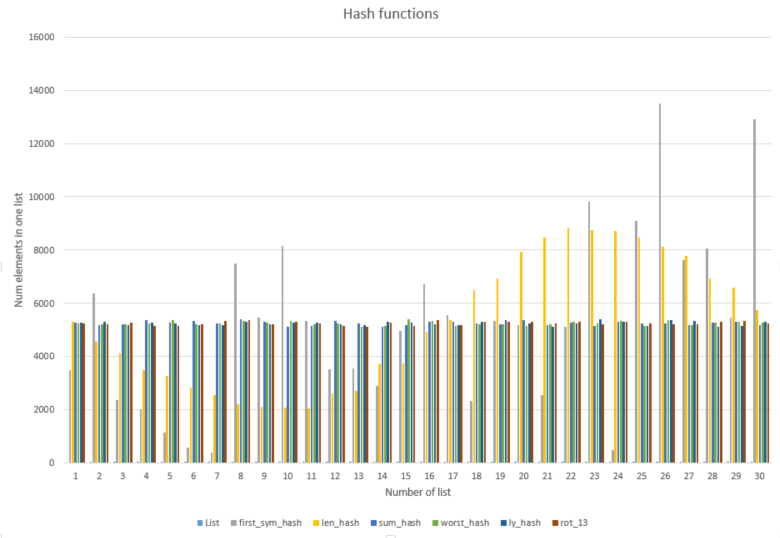
\includegraphics[scale=1]{2}}
	\caption{Измерение, сделанной без лучшей функции best-hash}
\end{figure}
\newpage
На данном графике по оси ординат отложено количество элементов в списке, а по оси абцисс номер списка. На легенде указано, кто какому цвету принадлежит, удивляет, только то, что не best-hash желтого цвета.
\newpage

\section*{Вывод}
Из данных графиков можно сделать вывод, что стоит пользоваться функциями rot-13, ly-hash and worst-hash (пример от Ильи Рудольфовича Дединского (Ded32))

\section*{Список литературы}
1. Язык программирования СИ, Брайан Керниган и Деннис Ритчи

2. \href{http://ded32.net.ru}{Дединский Илья Рудольфович}

Возможно, вы заходите заняться компутерной графикой и тогда вы сможете найти одну библиотеку, которая сможет вам помочь.

3. \href{https://www.google.ru}{Google}
\end{document}